%!TEX root = paper.tex
%%%%%%%%%%%%%%%%%%%%%%%%%%%%%%%%%%%%%%%%%%%%%%%%%%%%%%%%%%%%%%%%%%%%%%%%%%%%%%%%
\section{Background}
\label{sec:background}

Before looking at the fallacies in the literature, first some fundamental gaming terms and concepts need to be introduced. At their core video games are essentially feedback-directed real-time simulators. The game reads player input, updates the game state, and renders new screen contents. This loop repeats as long as the game is running. While the three parts are interrelated, and every component provides some form of input to the next, they may still proceed at their own intrinsic paces. The \textit{tickrate} governs the frequency of game state updates, and the \textit{framerate} determines the update rate of the output image. Popular examples for the tickrates of games servers include \SI{64}{\hertz} or \SI{128}{\hertz} for \textsc{CS:GO}, \SI{20}{\hertz} for \textsc{Minecraft}, or \SI{30}{\hertz} for \textsc{Dota 2}. Below the threshold of \textit{apparent motion} (about $16.67$ frames per per second) objects will appear as two distinct objects between two consecutive still images. Video games are more flexible but also much more demanding on the framerate than traditional media, whose framerates however at the lower end of motion perception. Video games have to target higher framerates, e.g., \SI{30}{\hertz}, \SI{60}{\hertz}, or even \SI{120}{\hertz}. This enables smoother camera and object movement and help increase the interactivity and reactivity as video games constantly require input on short time scales to which the game reacts and displays the feedback. Lag is a critically important factor for almost all games, as it governs the reaction time to in-game events. But it is often described solely on the basis of the network delay in an online game, neglecting other components that contribute to the lag, including the input device, the time to sample and process the input, the game engine and server and their tickrates, frame rendering time, and ultimately the time to display the frame on the monitor. Only if all sources are factored in the complete \textit{end-to-end lag} is captured, which can be highly variable. Fig.~\ref{fig:measurement-methods} depicts three distinct vantage points to measure the (partial) \gls{E2E} lag. However, only external methods can capture the complete lag.

\begin{figure}[!t]
    \centering
    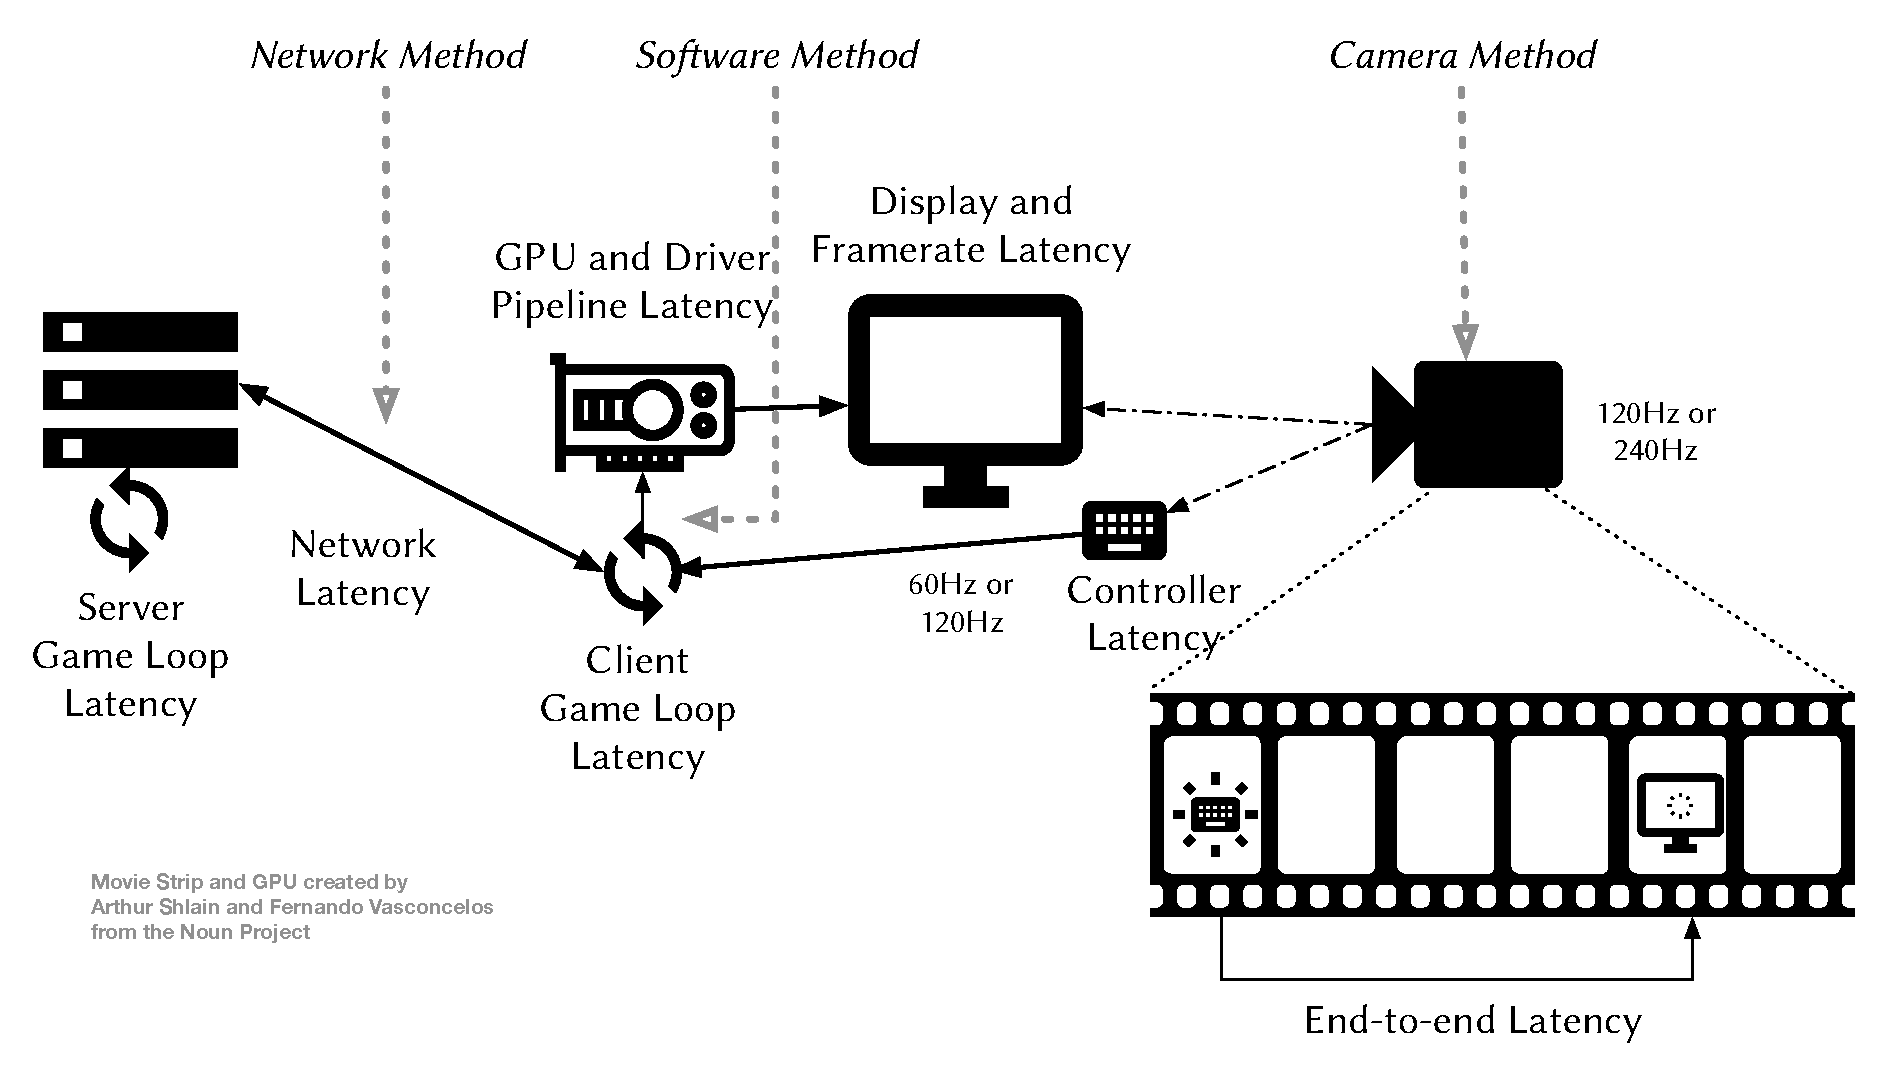
\includegraphics[width=1.0\columnwidth]{../../models/e2e-lag.pdf}
    \caption{Location of three measurement approaches to capture end-to-end lag in an online video game.}
\label{fig:measurement-methods}
\end{figure}


%%%%%%%%%%%%%%%%%%%%%%%%%%%%%%%%%%%%%%%%%%%%%%%%%%%%%%%%%%%%%%%%%%%%%%%%%%%%%%%%
\subsection{Related Work}

The outcome of user studies depends on a wide selection of factors (e.g., on the precise setup, the game, and the choice of players) which makes comparing their results quite difficult. Generalizing the game \acrshort{QoS} and \gls{QoE} assessments and their results has been a topic in past researches. E.g., correlating online cloud gaming quality with network \acrshort{QoS} (e.g. \cite{5976180} or \cite{6614351}). In order to avoid some of the issues with subjective user studies, other approaches examine the player objective performance through in-game metrics such as the game's highscore or the duration to achieve a certain task. The ``kills per minute'' of normal players in the \gls{FPS} \textsc{Quake 3} are, for example, investigated by \cite{1266180}, which sees a steady decline of this subjective performance metric when increasing the network delay. Finally, an ITU-T Recommendation \cite{mollertowards} concerning subjectively measuring video game \gls{QoE} is also in preparation, which discusses game-relevant \gls{QoS}-metrics as well as the selection of players and games.
